\section{Methods}
\label{sec:Methodes}


The optimization of the films was formulated as finding the minimum mass of \iso[6]{Li} for a given detector material necesary to fulfilll an interaction rate of \SI{2.5}{cps\per\nano\gram\iso[252]{Cf}} while mainting a intrisinic gamma rejection ratio of \num{1.e-6}.

\subsection{Design Parameters}
\label{sec:DesignParameters}
The design parameters were then:
\begin{itemize}
  \item The detector material. Materials with a high \iso{6}[Li] concentration will observe more neturons.
  \item The thickness of the detector material.
  \item The spacing of detector layers.
  \item The initial moderator thickness.
\end{itemize}

The intial moderator thickness was set at \SI{2.5}{\centi \meter}.
At this thickness around 10\% of the neutrons are thermalized (\todo{Cite my report}
\footnote{The thermal energy was chosen to be \SI{5}{\electronvolt}. The \isotope[6]{Li} neutron cross section as this energy is 67 barns. A sample containting 10\% \iso[6]{Li} and a density of\SI{1.0}{\gram \per \cubic \centi\meter} would then macroscopic cross section of \SI{0.67}{\per \centi\meter}, attenuating \SI{0.67}{\percent} of the incident flux in \SI{0.01}{ \centi\meter}
$$\Sigma = \frac{\rho N_A}{M}  \left ( n_1 \sigma_1 + n_2 \sigma_2 + n_3 \sigma_3 + \dots  \right ) $$}..

\begin{figure}
   \missingfigure{Fig on pg 68 of notebook}
\end{figure}

\begin{figure}
    \centering
    \begin{subfigure}[b]{0.45\textwidth}
        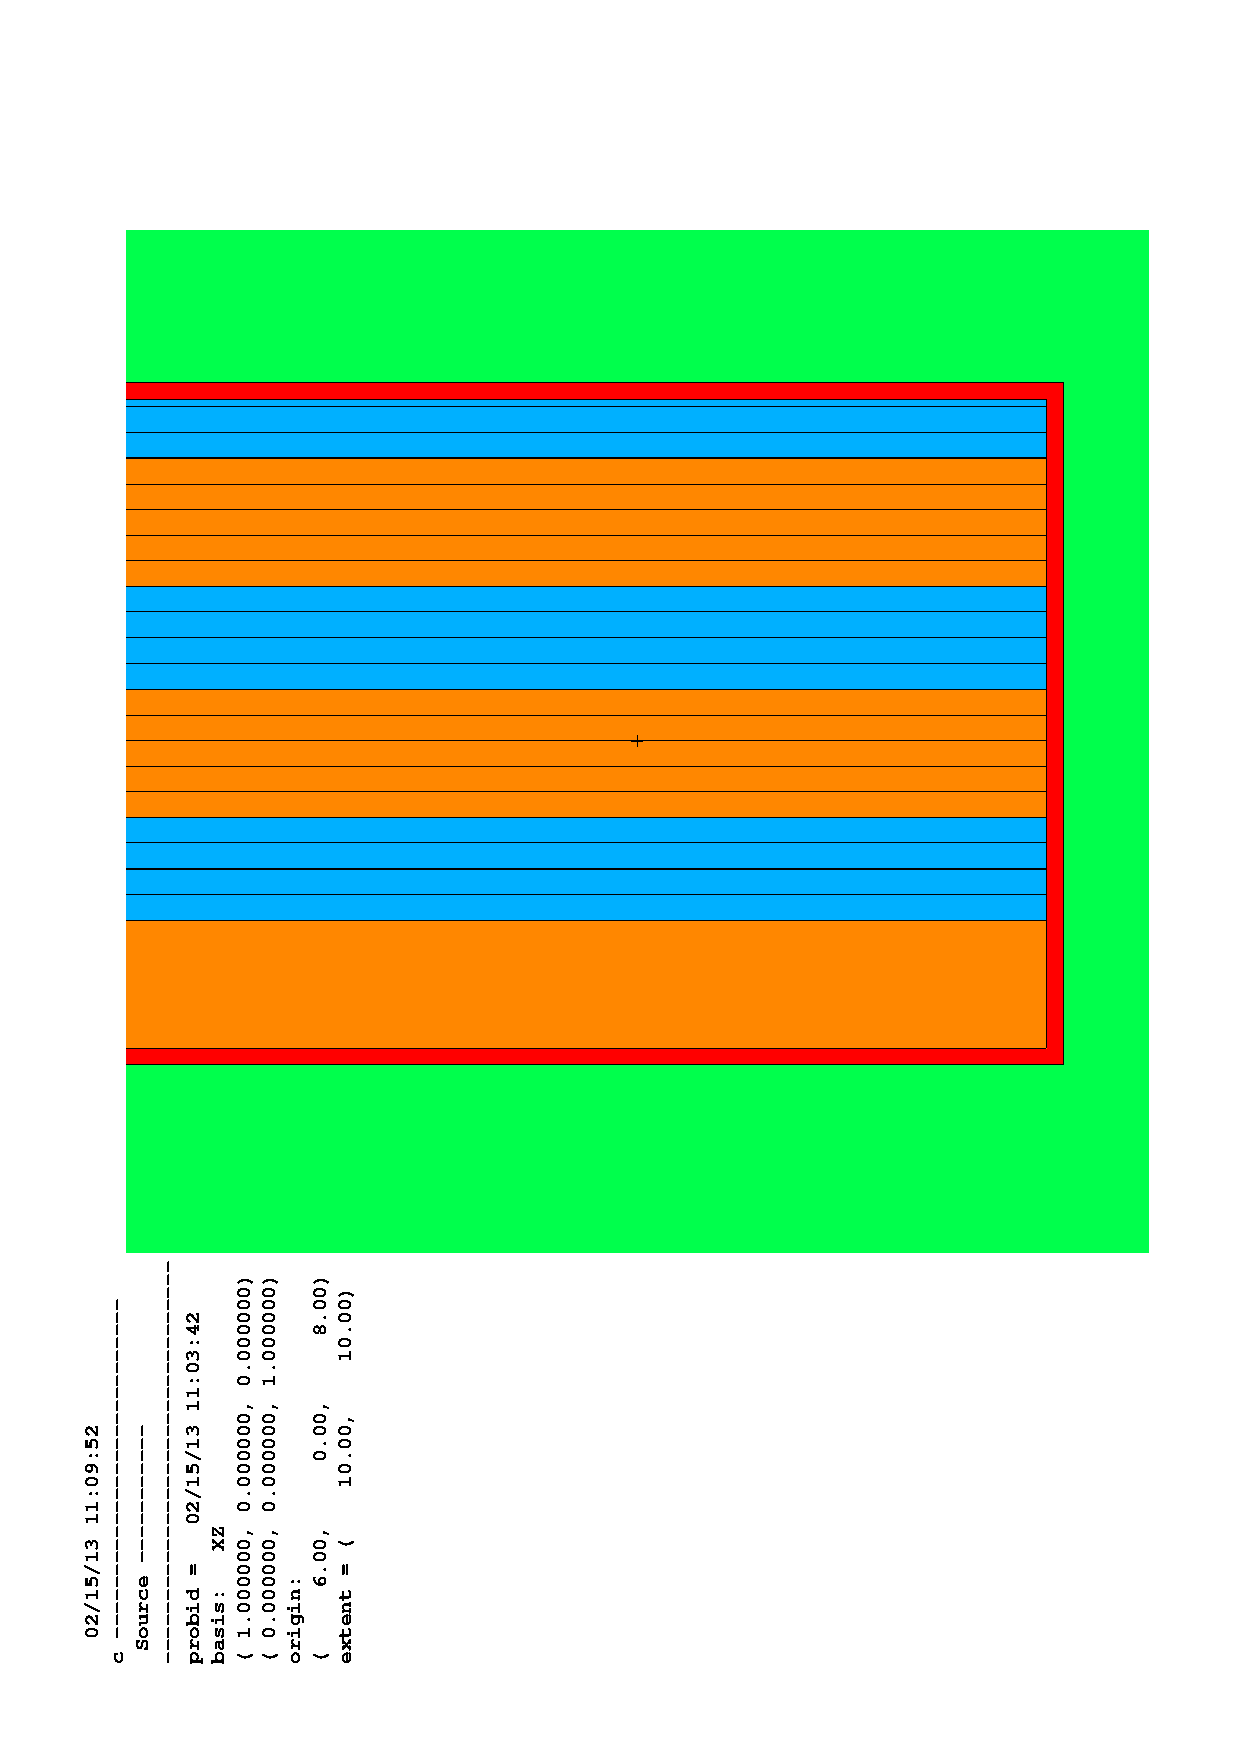
\includegraphics[width=\textwidth]{RPM8Opt_2_asm_2_cm.pdf}
        \caption{Two films per assembly with \SI{2}{\centi\meter} moderator spacing between assemblies}
    \end{subfigure}%
    ~
    \begin{subfigure}[b]{0.45\textwidth}
        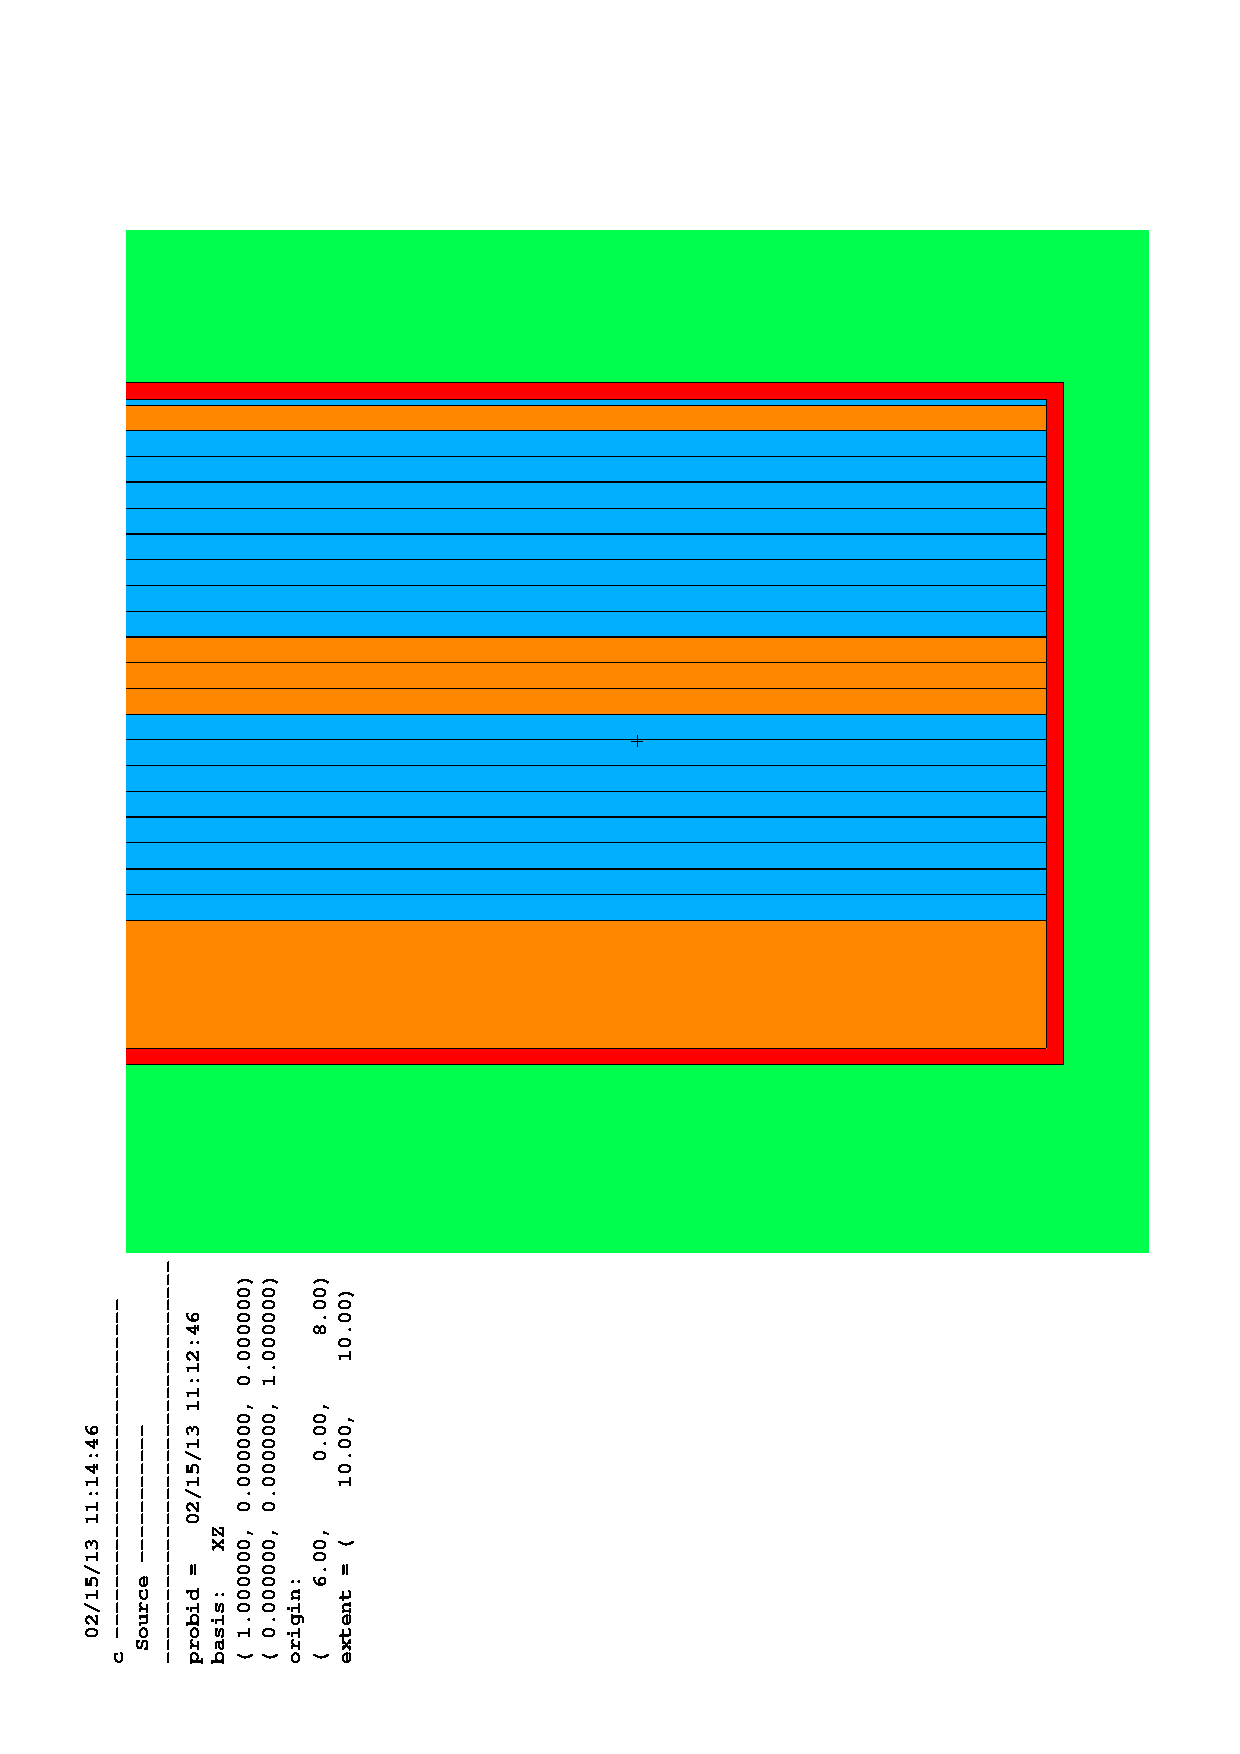
\includegraphics[width=\textwidth]{RPM8Opt_4_asm_1_cm.pdf}
        \caption{Four films per assembly with \SI{1}{\centi\meter} moderator spacing between assemblies}
    \end{subfigure}
    \caption{MCNPX rendering of layered geometry}
    \label{fig:MCNPXRendering}
\end{figure}
The optimization of the detector design is presented in two parts: a numerical approcach in which a matrix of detector spacing and assemblies are varied (Section ~\ref{sec:MCNPXMethods}, and a multi-variate optimization in which the paramters are fit to a functional form which is then optimized (Section ~\ref{sec:MVOptimization}.
\subsection{MCNPX Simulations}
\label{sec:MCNPXMethods}
A matrix of detector designs was simulated in MCNPX.
A generic script file was writen (Listing ~\ref{lst:MCNPXScript}) that was modified to include a user supplied number of detector assemblies, spacing between these assemblies, and initial moderator at the front of the assembly.


Two tallies were used in the MCNPX calcuations: the interaction rate tally (tally type 4) and the surface flux tally (type 2).
If the scalar flux is defiend as $\phi(\vec{r},E,t)=\int d\Omega \Phi(\vec{r},\hat{\Omega},E,t)$ the  interaction rate tally is the integral of all energies and directions of the scalar flux over a given volume, normalized by that volume ~\eqref{eqn:F4TallyDef}.
This quanity is then modified by an FM card which calculates quantities of the form $Q = C \int {\Phi(E) R_m(E) dE }$ where:
\begin{itemize}
    \item $C$ is a scalar normalization (density)
    \item $R_m(E)$ is the response function
    \item $\Phi(E)$ is the neutron flux
\end{itemize}
Simarly the surface flux is the integral over the entire surface (normalized by the surface area) of the scalar flux, as shown in \eqref{eqn:F2TallyDef}.
\begin{align}
    \label{eqn:F4TallyDef}
    \bar{\phi_V} = \frac{1}{V}\int dE \int dt \int dV \int d\Omega \AngularFlux
\end{align}
\begin{align}
    \label{eqn:F2TallyDef}
    \bar{\phi_S} = \frac{1}{A}\int dE \int dt \int dA \int d\Omega \AngularFlux
\end{align}

The FM card can modify any flux or current tally of the form $\int \psi (E) dE$ into $\int R(E)\psi(E) dE$, where $R(E)$ is the response function known to MCNP.
\subsection{1 D Transport Part}
The large detector and far away source suggest that the problem can be simplified into a one dimenionsal transport problem without suffering the accuracy of the solution.
As 1D deterministic transport is much faster than 3D Monte Carlo, 1D transport was explored in order to vary the problem parameters.

\subsection{Multivariate Optimization}
\label{sec:MVOptimization}

The multivariatie optimization problem was formulated as finding $\min_{\vec{x}} f (\vec{x})$ subject to contraints, where $f(\vec{x})$ is the response function.
